% Author: Seongjin Lee 
% Hanyang University, Seoul, Korea 
% esos.hanyang.ac.kr 
% 2016-09-20
% note: some slides are adopted from  \url{www.cs.stevens.edu/~jschauma/631A/}
% https://github.com/resourceful/lecture_sysprog/

\documentclass[newPxFont,sthlmFooter,nooffset]{beamer}
\usepackage{kotex}
%\usetheme{sthlm}
\usepackage{../beamer_template/beamerthemesthlm}
\hypersetup{pdfauthor={Seongjin Lee (insight@hanyang.ac.kr)},
            pdfsubject={Lecture Note: System Programming},
            pdfkeywords={Lecture Note, System Programming, class, undergraduate},
            pdfmoddate={D: \pdfdate},
            pdfcreator={Seongjin Lee}}

%\setbeamertemplate{footline}[text line]{%
%    \parbox{\linewidth}{\vspace*{-8pt} \insertsectionhead  \hfill\insertshortauthor\hfill\insertpagenumber}}
%\setbeamertemplate{navigation symbols}{}




\title{System Programming}
\subtitle{Week 12: Working with others and Regular Expressions}
\author[SJL]{Seongjin Lee}
\institute{\href{mailto:insight@hanyang.ac.kr}{insight@hanyang.ac.kr}\\\url{http://esos.hanyang.ac.kr}\\Esos Lab. Hanyang University}
\date{2016-11-16} 

\begin{document}



\frame[plain]{\titlepage} 

\frame[t]{\frametitle{Table of contents}\tableofcontents} 


%---------------------------------------------------------



\begin{frame}[t]
  \frametitle{Introduction}

Working with others 

In this lecture we will cover version control system and Regular Expressions
\begin{itemize}
\item Subversion or SVN
\item GIT
\item Regular Expressions
\end{itemize}
\end{frame}

\section{Terminology}

\begin{frame}[t]
  \frametitle{The History}
{\footnotesize
  \begin{table}[h]
    \centering
    \begin{tabular}{l | l | m{2cm} | m{2cm} | m{3cm}}
      Generation & Networking & Operations & Concurrency & Examples \\ \hline \hline
First & None & One file at a time & Locks & RCS, SCCS \\ \hline
Second & Centralized & Multi-file & Merge Before Commit & CVS, Subversion, SourceSafe, Team Foundation Server \\ \hline
Third & Distributed & Change sets & Commit before Merge & Bazzar, Git, Mecucial
    \end{tabular}
  \end{table}
}

The history of version control is very long (about forty years)
\begin{itemize}
\item It steadily moved towards to support more concurrency
\item First generation used locks to manage concurrency – one person at a time
\item Second generation is more permissive about simultaneous modification – merge before commit
\item Third generation separates merge and commit operations
\end{itemize}
\end{frame}


\begin{frame}[t]
  \frametitle{Basic Terminology}
\textbf{Repository} is a official place to store the work
\begin{itemize}
\item Keeps track of tree of files and directories
\item More importantly it contains history
\item Create operation makes a new repository
\end{itemize}
\bigskip

\begin{center}
  \textbf{Repository = File system $\times$ Time}
\end{center}

\end{frame}



\begin{frame}[fragile,t]
  \frametitle{Basic Terminology cnt'd}
\textbf{Checkout} creates a working copy of existing repository to local storage

\textbf{Working copy} is current copy of the project in the local stroage

\begin{itemize}
\item Records timestamp on the working file
\item Records the version number of the repository file (to note the
  start)
\item Keeps complete copy of the retrieved file
\end{itemize}

\begin{verbatim}
     WorkCycleFromStart:
          make a working copy from repository

     WorkCycle:
          modify working copy
          update the repository

     GOTO WorkCycle
\end{verbatim}


\end{frame}


\begin{frame}[t]
  \frametitle{Basic Terminology cnt'd}
\textbf{Commit} applies modification in the working copy to the repository as a new change set

\begin{itemize}
\item Several others modify the working copy and add an operations to a pending changeset list
\item Pending changeset – a place where changes wait to be commited
\item Commit operation takes the pending changeset and makes it to create a new version of the tree in the repository
\item Operations are atomic (all or nothing)
\end{itemize}


\end{frame}


\begin{frame}[t]
  \frametitle{Basic Terminology cnt'd}

\texttt{Update} renews the working copy with respect to the repository
\begin{itemize}
\item Make working copy up-to-date
\item Apply changes from the repository, merge them with any changes on the working copy

\end{itemize}


\end{frame}


\begin{frame}[t]
  \frametitle{Basic Terminology cnt'd}
\textbf{ADD} – add a file or directory for version control
\begin{itemize}
\item After add they become part of the pending changeset
\end{itemize}


\textbf{EDIT} – modify a file
\begin{itemize}
\item Edit operation does not involve the VCS
\end{itemize}


\textbf{DELETE} – delete a file or directory
\begin{itemize}
\item Remove a file or directory from the repository
\item Immediately delete the working copy of the file, but they are left in pending changeset
\item File / directory in the repository is not really deleted; just making a new tree w/o them
\end{itemize}


\end{frame}


\begin{frame}[t]
  \frametitle{Basic Terminology cnt'd}
\textbf{RENAME} – rename a file or directory
\begin{itemize}
\item Some of the earlier tools had no support for it; so, should check how your VCS works
\end{itemize}



\textbf{MOVE} – move a file or directory
\begin{itemize}
\item Move file or directory from one place in the tree to another
\item Operation is added to the pending changeset
\end{itemize}

\textbf{STATUS} – list the modifications that have been made to the working copy
\begin{itemize}
\item It shows the list of of pending changeset
\end{itemize}




\end{frame}


\begin{frame}[t]
  \frametitle{Basic Terminology cnt'd}
\textbf{DIFF} – shows the details of the modifications that have been made to the working copy
\begin{itemize}
\item Status for list and diff for what exactly have been changed
\item How it prints out the differences is VCS dependent
\end{itemize}


\textbf{REVERT} – undo modifications that have been made to the working copy
\begin{itemize}
\item Throw away all your pending changeset and the return the working
  copy to the way it was just after the checkout
\end{itemize}

\textbf{LOG} – show the history of changes to the repository
\begin{itemize}
\item Keeps track of every version and changes made to the project including Who, When, and What
\end{itemize}

\end{frame}


\begin{frame}[t]
  \frametitle{Basic Terminology cnt'd}

\textbf{TAG} – associate a meaningful name with a specific version in the repository
\begin{itemize}
\item To mark a specific instant in the history of the repository with
  meaningful name
\end{itemize}


\textbf{BRANCH} – create another line of development
\begin{itemize}
\item To fork off into two different directories
\end{itemize}

\textbf{MERGE} – apply changes from one branch to another
\begin{itemize}
\item Used branch to enable the development to diverge, merge is to
  converge again
\end{itemize}

\end{frame}



\begin{frame}[t]
  \frametitle{Basic Terminology cnt'd}
\textbf{RESOLVE} – handle conflicts resulting from a merge
\begin{itemize}
\item VERY IMPORTANT
\end{itemize}


\textbf{LOCK} – prevent other people from modifying a file
\begin{itemize}
\item Not all have this feature
\end{itemize}
\end{frame}

\section{Subversion}



\begin{frame}[t]
  \frametitle{Installing SVN}

  \begin{itemize}
  \item For linux       \texttt{ apt-get install subversion libapache2-svn}
  \item For mac - Build using source code or check if it has one
  \end{itemize}

To check version of installed SVN
\begin{itemize}
\item \texttt{svn --version}
\end{itemize}
\end{frame}


\begin{frame}[fragile,t]
  \frametitle{Second Generation: SVN}
It is a centralized version control system

\begin{verbatim}
  mkdir projectA
  svnadmin create projectA/trunk
  svnserver -d --root=/Users/James/projectA
\end{verbatim}

\end{frame}


\begin{frame}[fragile,t]
  \frametitle{Second Generation: SVN cnt'd}

\begin{verbatim}
  // checkout a repository
  svn checkout http://PROJECT.URL/projectA

  // add a file you want to manage in svn
  svn add YOURFILE

  // see what is changed and managed
  svn status

  // commit your work to repository
  svn commit -m "LOG CONTENT"

  // see records of changes
  svn log --verbose | more
\end{verbatim}

\end{frame}


\begin{frame}[fragile,t]
  \frametitle{Second Generation: SVN cnt'd}
Merge changes to the working copy : \texttt{svn update}

\begin{verbatim}
svn update

Select: (p) postone, (df) diff-full,  (e) edit,  (r) resolved,
        (mc) mine-conflict,  (tc) theirs-conflict, 
        (s) show all options: 
\end{verbatim}
\begin{itemize}
\item Postpone – deal with the conflict later
\item Resolved – mark it as solved
\begin{itemize}
\item \texttt{svn resolve –accept=working}
\end{itemize}
\item Mine-conflict – use my version as new
\item Theirs-conflict – use the repository as new
\end{itemize}
\end{frame}


\begin{frame}[fragile,t]
  \frametitle{Second Generation: SVN cnt'd}
\begin{verbatim}
  // see what is changed in your file
  svn diff -r 1 YOURFILE
\end{verbatim}


Example of text with conflict
\begin{verbatim}

<<<<<<<< .mine
Some text is introduced in this line
This is what James wrote
========
Some different contents in this line
This is what Abraham wrote
>>>>>>>> .r4
\end{verbatim}


\end{frame}


\begin{frame}[t]
  \frametitle{Second Generation: SVN cnt'd}
\texttt{svn help} gives minimal usage of commands

The commands are 

\begin{itemize}
\item create
% \item checkout
% \item commit
% \item update
% \item add
\item delete
\item rename
\item move
% \item status
% \item diff
\item revert
% \item log
\item tag
\item branch
\item merge
\item resolve
\end{itemize}

\end{frame}


\section{GIT}



\begin{frame}[t]
  \frametitle{Third Generation Background: GIT}
It is distributed or decentralized version control system

Synchronizing the local and the remote
\begin{itemize}
\item \textbf{PUSH} – copy changesets from a local repository instance to a remote one
\item \textbf{PULL} – copy changesets from a remote repository instance to a local one
\item Note that not all changes on the local is same as that on the remote
\end{itemize}


\end{frame}



\begin{frame}[t]
  \frametitle{Backgrounds}
Directed Acyclic Graph (DAGs)
\begin{itemize}
\item Ability to push and pull changesets between multiple instances of the same repository comes from a design model called DAG
\item Consists of Node, directed edge, root node, leaf node
\item Node – represents one revision of the entire repository tree
\item Directed edge – shows relationship between nodes
\end{itemize}
\end{frame}

\begin{frame}[t]
  \frametitle{Backgrounds: DAGs}
Repository history as a line
\begin{itemize}
\item Fork latest version
\item Modify
\item Check back in
\end{itemize}
\begin{figure}[h]
  \centering
  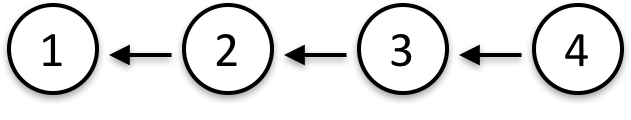
\includegraphics[width=0.5\linewidth]{figures/fig1}
\end{figure}


\end{frame}

\begin{frame}[t]
  \frametitle{Backgrounds: DAGs}
Somebody else does the same
\begin{itemize}
\item Before I make change to version 3 somebody else already made
  version 4
\end{itemize}


\begin{figure}[h]
  \centering
  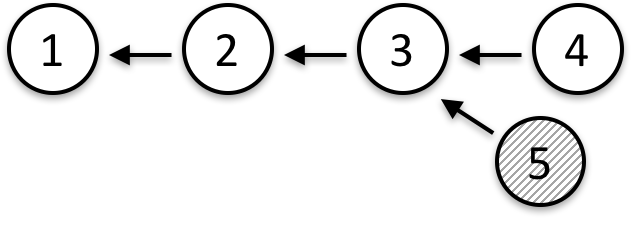
\includegraphics[width=0.5\linewidth]{figures/fig2}
\end{figure}


\end{frame}

\begin{frame}[t]
  \frametitle{Backgrounds: DAGs}
REMEMBER to commit before merge
\begin{figure}[h]
  \centering
  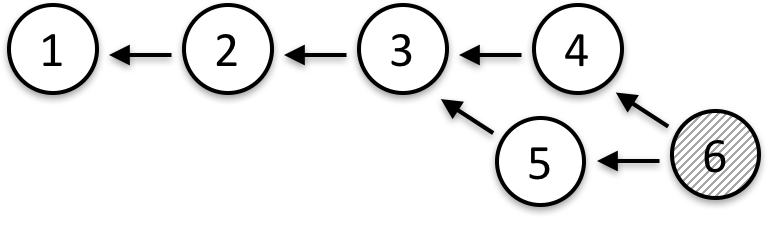
\includegraphics[width=0.5\linewidth]{figures/fig3}
\end{figure}

Benefit of having DAG model
\begin{itemize}
\item Everything is not linear
\item Flexible and expressive
\end{itemize}


\end{frame}


\begin{frame}[t]
  \frametitle{Advantages of Distributed Version Control System}
It gives private workspace for the whole repository

It is fast

It works offline

It scales out and up

\end{frame}



\begin{frame}[t]
  \frametitle{Work Flow }
\begin{figure}[h]
  \centering
  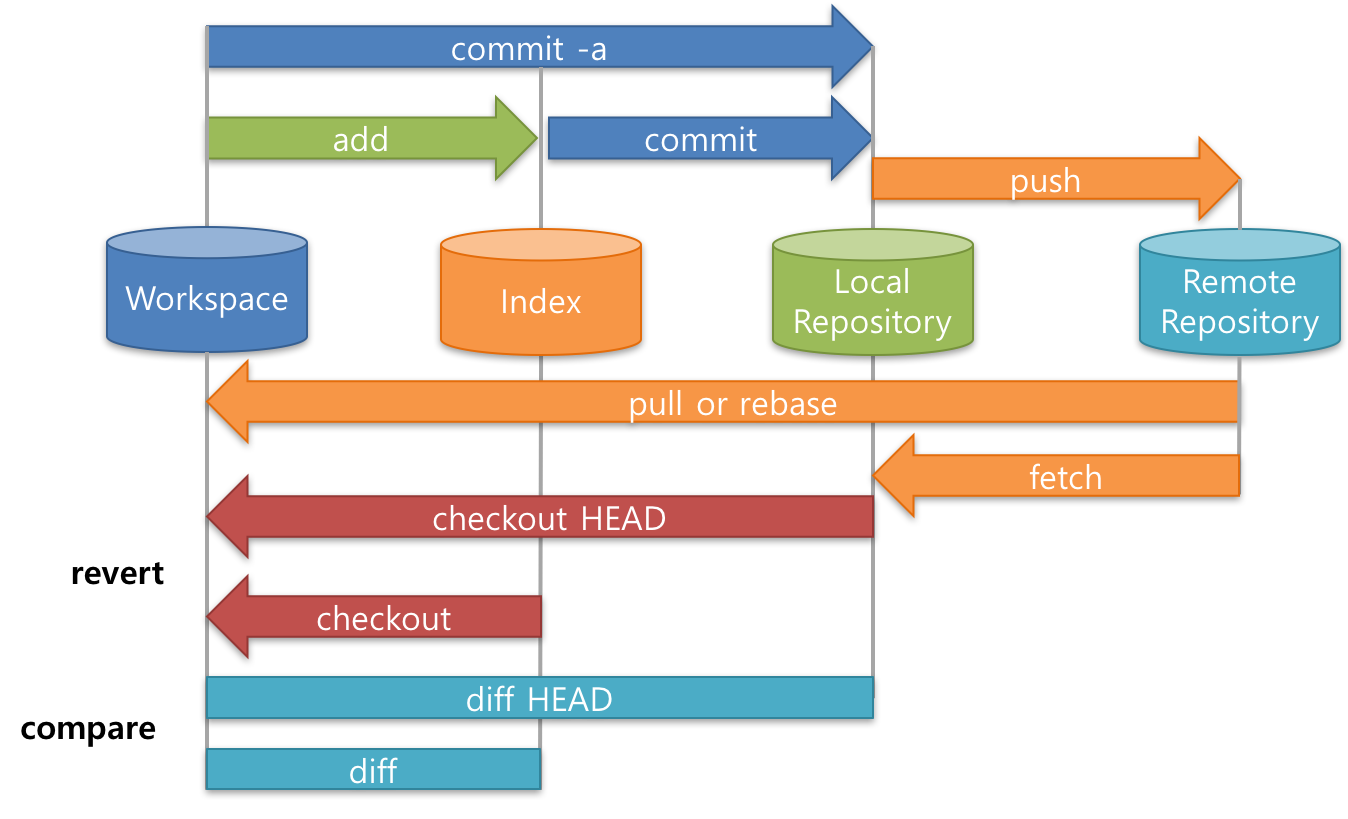
\includegraphics[width=\linewidth]{figures/fig4}
\end{figure}


\end{frame}

\begin{frame}[t]
  \frametitle{File Management }
It keeps the delta of the object

\begin{figure}[h]
  \centering
  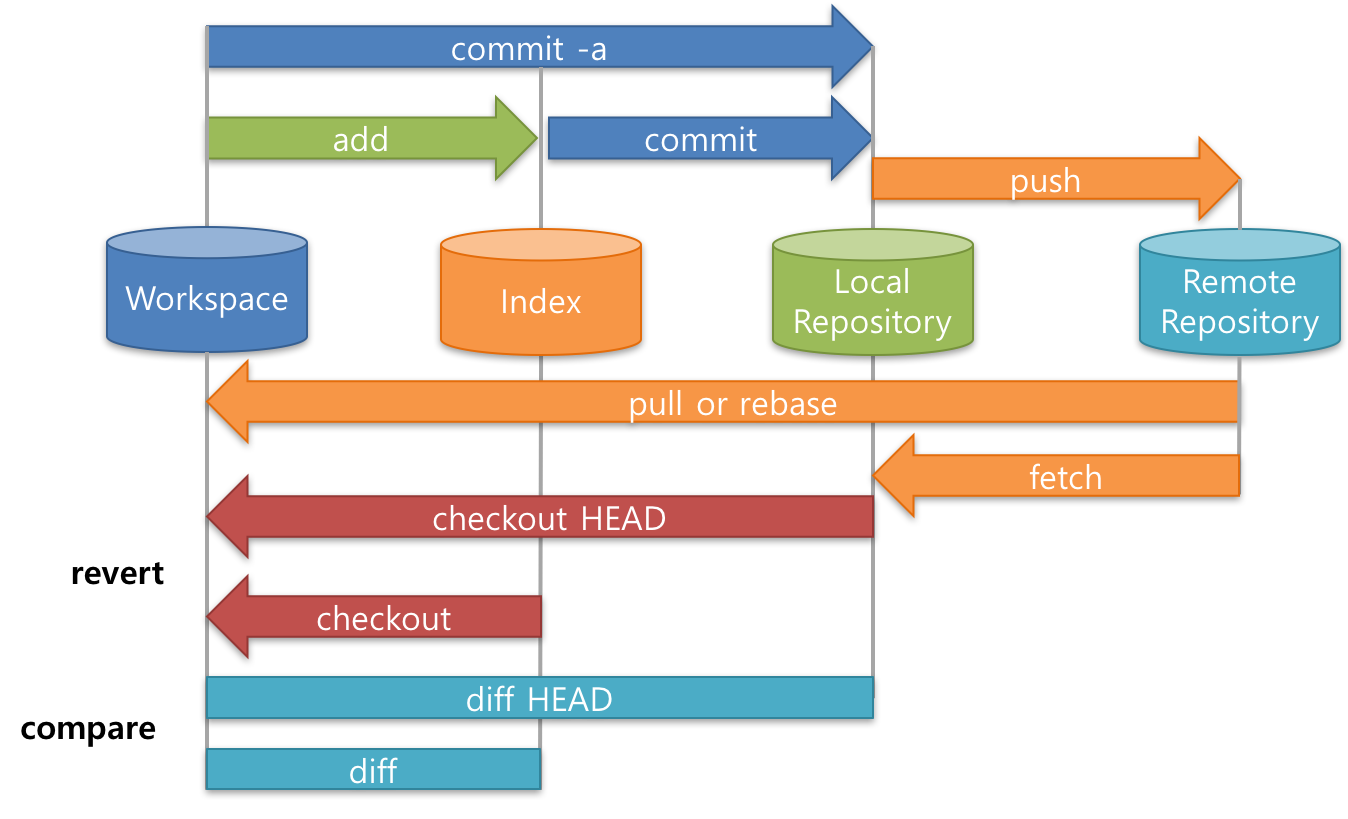
\includegraphics[width=\linewidth]{figures/fig4}
\end{figure}

\end{frame}

\begin{frame}[t]
  \frametitle{Installing GIT}

  \begin{itemize}
  \item For linux        \texttt{apt-get install git}
  \item For mac         \url{http://git-scm.com/download/mac}
  \end{itemize}

To check version of installed GIT
\begin{itemize}
\item \texttt{git --version}
\end{itemize}
\end{frame}


\begin{frame}[fragile,t]
  \frametitle{Basics }
If you have a git server already installed on the local PC
\begin{verbatim}
mkdir Project-with-git
cd Project-with-git
git init -bare Project-with-git
\end{verbatim}


\end{frame}

\begin{frame}[fragile,t]
  \frametitle{Basics }

If you have an account in github.com
\texttt{vi ~/.gitconfig}
\begin{verbatim}
[user]
   name = YOURID
   email = YOUREMAIL
\end{verbatim}

\texttt{git clone address}
\end{frame}

\begin{frame}[fragile,t]
  \frametitle{Basics }
\begin{verbatim}
git pull

git add YOURFILE

git commit -m "LOG"

git push
\end{verbatim}
\end{frame}

\begin{frame}[fragile,t]
  \frametitle{Basics}
Example text with conflicts

\begin{verbatim}
<<<<<<<< HEAD
Some text is introduced in this line
This is what James wrote
========
Some different contents in this line
This is what Abraham wrote
>>>>>>>> b30hf32hfaohf8dhaf8a
\end{verbatim}
\end{frame}





\section{Regular Expression}

\begin{frame}[fragile,t]
  \frametitle{Search for Strings: \texttt{grep} Overview}

\begin{block}{Usage}
\texttt{grep\footnote{set \texttt{alias grep='grep --color=auto'} in .bash\_profile} pattern filename}
\end{block}

\bigskip
Examples
\begin{itemize}
\item \texttt{grep hello world}
\item \texttt{grep ``hello world''}
\item \texttt{grep ``h.llo''}
\item \texttt{grep ``h*llo''}
\item \texttt{grep ``hello $\backslash|$ world''}
\end{itemize}
\end{frame}

\begin{frame}[t]
  \frametitle{\texttt{grep -E} for extended \texttt{grep} with regular
    expression}
Download sample text from \url{http://www.ats.ucla.edu/stat/examples/chp/p176.txt} (use \texttt{wget} to download)
\bigskip
Examples 
\begin{itemize}
\item 2 to 3 vowels: \texttt{grep -E ``[aeiou]\{2,3\}'' brain.txt}
\item OR cases
  \begin{itemize}
  \item  \texttt{grep -E ``A[sf]*'' brain.txt}
  \item \texttt{grep -E ``Asian $\backslash|$ African''}
  \end{itemize}
\end{itemize}
\end{frame}

\begin{frame}[t]
  \frametitle{\texttt{grep -E} for extended \texttt{grep} with regular
    expression}
Download a sample text from \url{https://www.gnu.org/licenses/gpl.txt
}

\bigskip

yet another example of OR search
\begin{itemize}
\item  \texttt{grep -E ``(GPL$\backslash|$ General Public License)'' gpl.txt}
\end{itemize}

\bigskip
Meta characters: begin with capital letter and end with period
\begin{itemize}
\item  \texttt{grep -E ``$^{\wedge}$[A-Z].*$\backslash$.\$'' gpl.txt }
\end{itemize}
\end{frame}


\begin{frame}[t]
  \frametitle{Examples cnt'd}
Optional group of string
\begin{itemize}
\item \texttt{grep -D ``([cC]opy)?right'' gpl.txt}
\end{itemize}

\bigskip

Words with 16 to 20 characters
\begin{itemize}
\item \texttt{grep -E ``[[:alpha:]]\{16,20\}'' gpl.txt}
\end{itemize}

\bigskip

Groups are used in
\begin{itemize}
\item repeating set: 
  \begin{itemize}
  \item \texttt{(Love)\{5\}} matches \texttt{LoveLoveLoveLoveLove}
  \item Love\{5\} matches: \texttt{Loveeeee}
  \end{itemize}
\item Back referencing usually used in replacing. It is also called capturing group
  \begin{itemize}
  \item \texttt{grep -E ``foo(bar)?(baz)(quz)'' }
  \end{itemize}
\end{itemize}
\end{frame}

\begin{frame}
  \frametitle{Review with interactive excercises}

Interactive excercises: 
  \url{https://regexone.com/lesson/introduction_abcs}

Using regular Expression in Vim
  \url{http://vimregex.com/}

\end{frame}

%---------------------------------------------------------
\begin{comment}
\section{Last Words}

\begin{frame}[t]
  \frametitle{Last Words}

\begin{itemize}
\item 
\end{itemize}
\end{frame}

\end{comment}

\end{document}
